\documentclass{beamer}
%
% HOWTO Compile Presentation:
%
%    pdflatex introduction-to-git.tex
%
% Some Notes:
%
%    Add git fetch example in next iteration. 
%    Maybe add pull request example too.
%
\usepackage{amsmath}
\usepackage{amssymb}
\usepackage{centernot}
\usepackage{graphics}
\usepackage{hyperref}
\usepackage{listings}
\usepackage{setspace}

\usepackage{textcomp}

\usepackage{tikz}

\newcommand{\shrug}[1][]{%
\begin{tikzpicture}[baseline,x=0.8\ht\strutbox,y=0.8\ht\strutbox,line width=0.125ex,#1]
\def\arm{(-2.5,0.95) to (-2,0.95) (-1.9,1) to (-1.5,0) (-1.35,0) to (-0.8,0)};
\draw \arm;
\draw[xscale=-1] \arm;
\def\headpart{(0.6,0) arc[start angle=-40, end angle=40,x radius=0.6,y radius=0.8]};
\draw \headpart;
\draw[xscale=-1] \headpart;
\def\eye{(-0.075,0.15) .. controls (0.02,0) .. (0.075,-0.15)};
\draw[shift={(-0.3,0.8)}] \eye;
\draw[shift={(0,0.85)}] \eye;
% draw mouth
\draw (-0.1,0.2) to [out=15,in=-100] (0.4,0.95); 
\end{tikzpicture}}

\lstset{language=bash,basicstyle=\ttfamily\small\color{black}}

\title{An Introduction to \texttt{git} (and GitHub): \\
       \small A Distributed Version Control System}
\author{Marty Kandes, Ph.D. \\ \ \\
 \small HPC User Services Group \\
        San Diego Supercomputer Center \\
        University of California, San Diego}
\date{\small SDSC Summer Institute 2019\\
             Monday, August 5th, 2019 \\
             10:30AM - 12:00PM PDT}

\begin{document}
\maketitle

\begin{frame}
   \frametitle{About Me}
   \begin{itemize}
      \setlength\itemsep{1.0em}
      \item Background in Computational Atomic Physics
      \item HPC user who got into HPC infrastructure while finishing PhD
      \item Joined HPC User Services Group @ SDSC in April 2017
      \item Previously worked for the Distributed High-Throughput 
         Computing Group @ SDSC and the Open Science Grid
      \item I am most definitely \textbf{not} a \texttt{git} expert. 
   \end{itemize}
\end{frame}

\begin{frame}
   \frametitle{Today's Session}
   \begin{itemize}
      \setlength\itemsep{1.0em}
      \item An Overview of Version Control
      \item About \texttt{git}
      \item Getting Started with \texttt{git}
      \item Working with \texttt{git}
      \item Getting Started with GitHub
      \item Summary and Conclusion
      \item Q\&A
   \end{itemize}
\end{frame}

\begin{frame}
   \frametitle{An Overview of Version CON-WHAT?}
   \begin{figure}[htbp]
      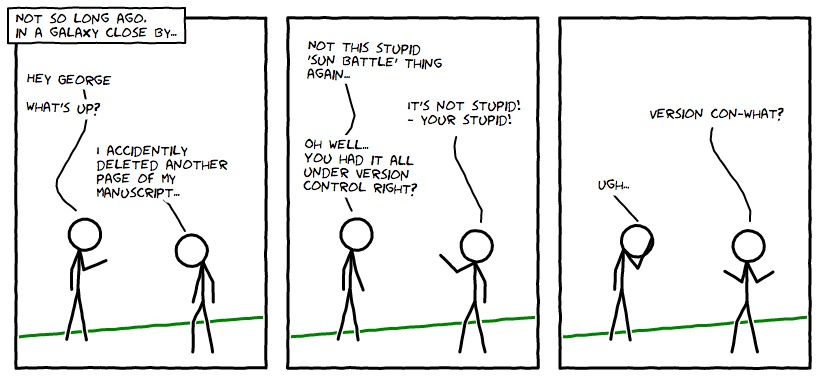
\includegraphics[width=1.0\textwidth]{images/version-control-xkcd.jpg}
   \end{figure}
\end{frame}

\begin{frame}
   \frametitle{What is version control?}
   \textit{Version control} is the process of recording and managing 
   changes to a file or set of files over time so that you can recall 
   specific versions later, if needed.
\end{frame}

\begin{frame}
   \frametitle{What do we version control?}
   The files we're typically interested in being version 
   controlled are \textit{software source code} files. However, you can 
   version control almost any type of file.
   
\end{frame}

\begin{frame}
   \frametitle{What \textit{should} we version control?}
   \textit{``In practice, everything that has been created manually should be
   put in version control, including programs, original field 
   observations, and the source files for papers.''} 
   \\ \ \\
   \ \ \ \ \ \ \ \ \ \ \ \ \ \ \ \ \ \ \ \ \ \ \ \ \ \ \ \ 
   Best Practices for Scientific Computing \\
   \ \ \ \ \ \ \ \ \ \ \ \ \ \ \ \ \ \ \ \ \ \ \ \ \ \ \ \ 
   Wilson et al. 2012 (arXiv:1210.0530)
\end{frame}

\begin{frame}
   \frametitle{Have you used version control before?}
   \begin{figure}[htbp]
      
\includegraphics[width=0.5\textwidth]{images/version-control-phdcomics.png}
   \end{figure}
\end{frame}

\begin{frame}
   \frametitle{Yes, yes I have ...}
   \begin{figure}[htbp]
      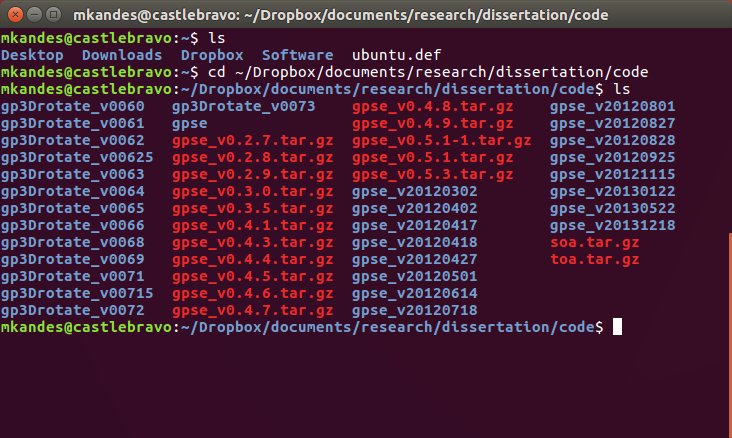
\includegraphics[width=1.0\textwidth]{images/bad-version-control.png}
   \end{figure}
   \url{https://github.com/mkandes/gpse}
\end{frame}

\begin{frame}
   \frametitle{What is a version control system?}
   \begin{itemize}
      \setlength\itemsep{1.0em}
      \item A \textit{version control system} (VCS) is a type of software 
         tool that helps record and manage the changes you make to the 
         file or set of files you want version controlled.
      \item Version control systems keeps track of \textit{every} 
         modification you make to the files being tracked in a special 
         kind of database.
      \item If a mistake is made, you can then turn back the clock and 
         compare earlier versions of the files to help fix the mistake. 
   \end{itemize}
\end{frame}

\begin{frame}
   \frametitle{Example: Apple's Time Machine}
   \begin{figure}[htbp]
      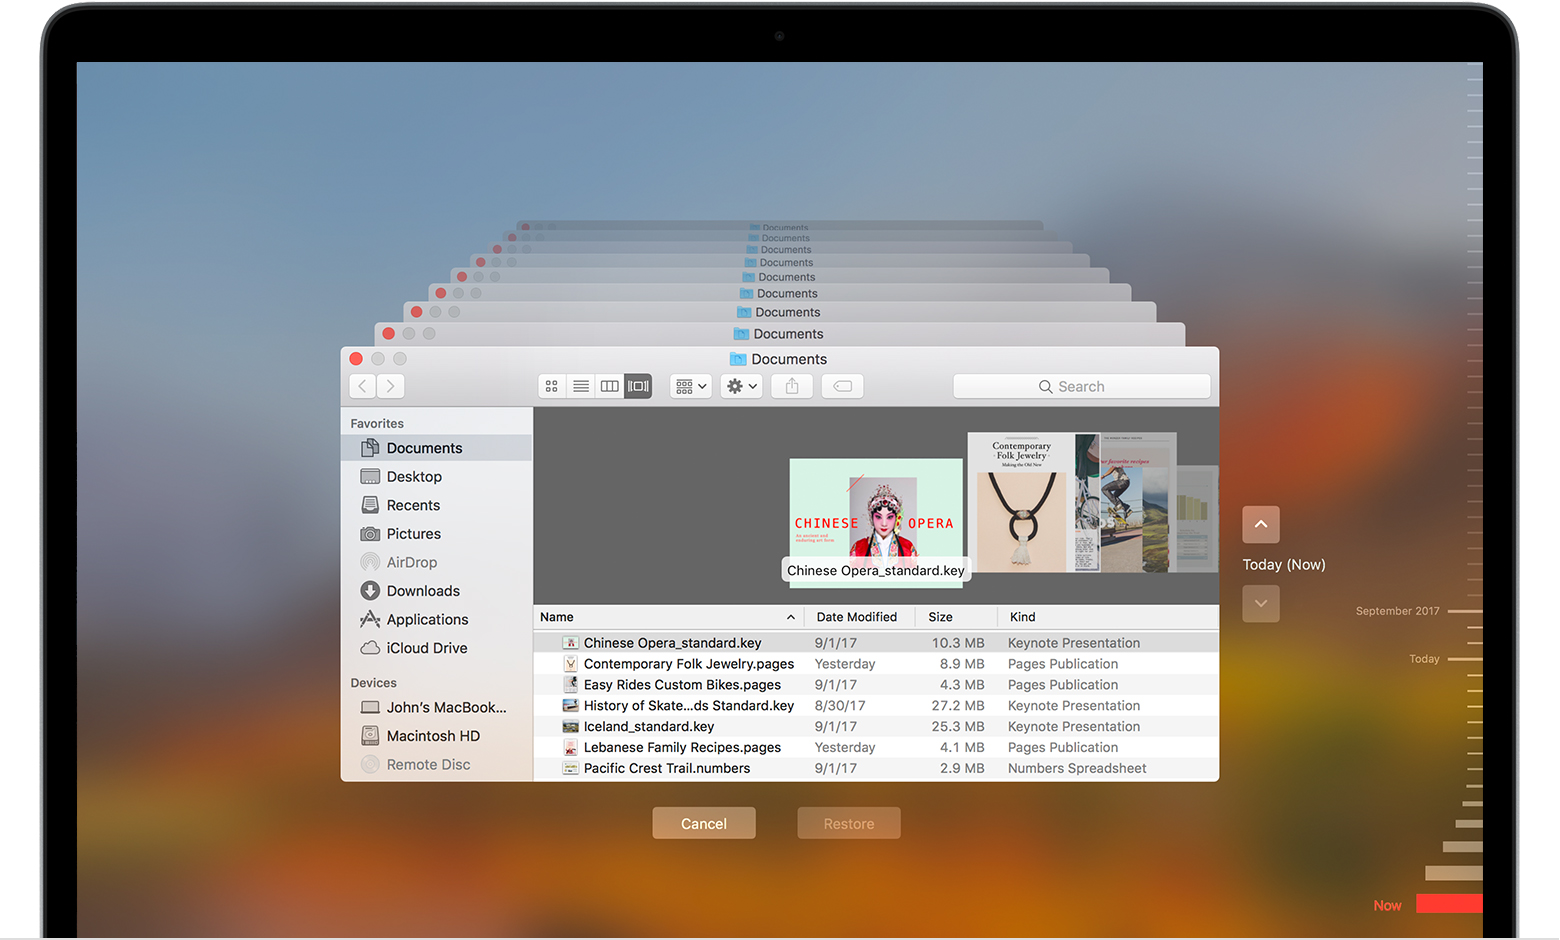
\includegraphics[width=1.0\textwidth]{images/macos-high-sierra-time-machine-documents.jpg}
   \end{figure}
\end{frame}

\begin{frame}
   \frametitle{Example: Dropbox}
   \begin{figure}[htbp]
      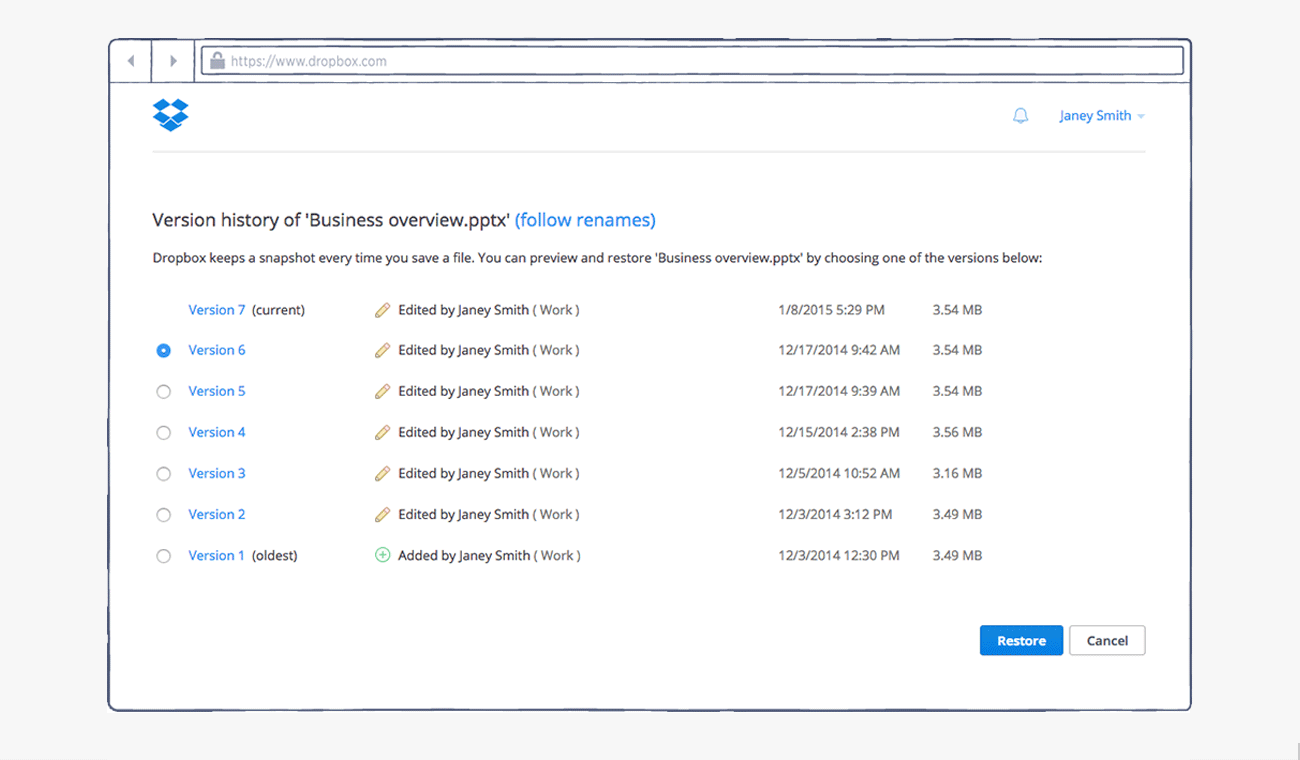
\includegraphics[width=1.0\textwidth]{images/dropbox_view_version_history.png}
   \end{figure}
\end{frame}

\begin{frame}
   \frametitle{Example: Microsoft Word's Track Changes}
   \begin{figure}[htbp]
      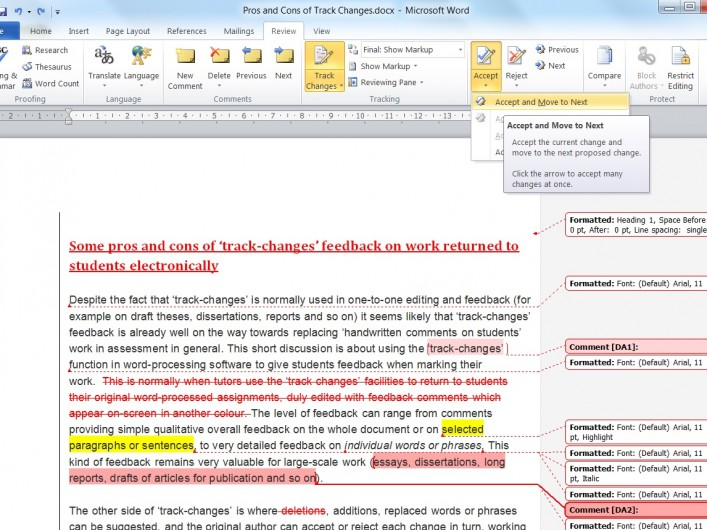
\includegraphics[width=0.9\textwidth]{images/ms-word-track-changes.jpg}
   \end{figure}
\end{frame}

\begin{frame}
   \frametitle{Example: Wikipedia's View History}
   \begin{figure}[htbp]
      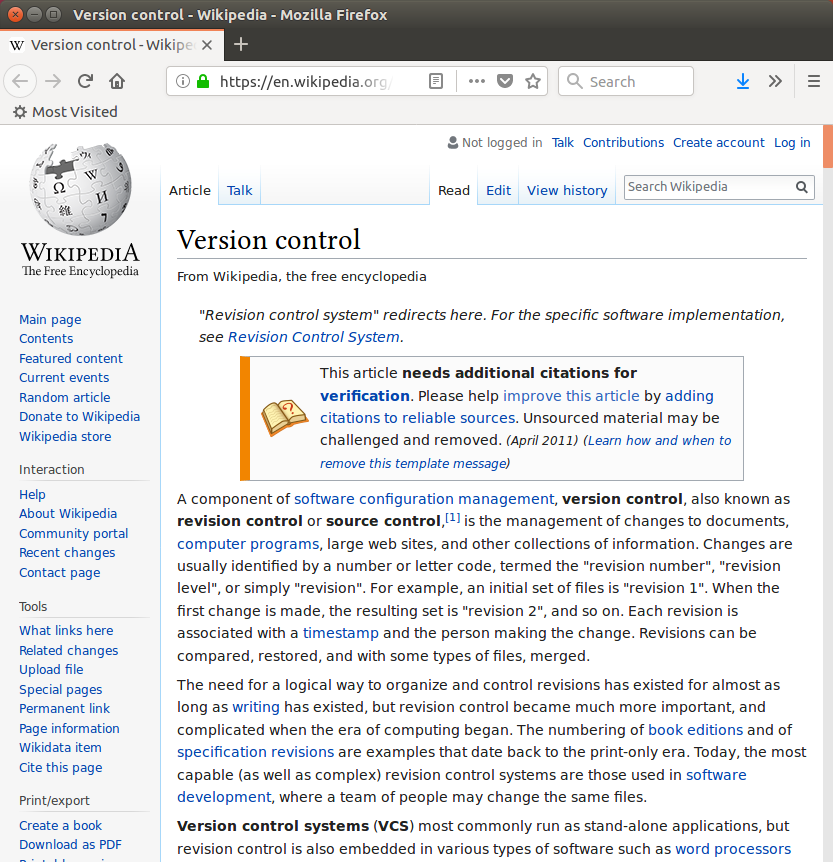
\includegraphics[width=0.9\textwidth]{images/version-control-wikipedia.png}
   \end{figure}
\end{frame}

\begin{frame}
   \frametitle{Example: Wikipedia's View History}
   \begin{figure}[htbp]
      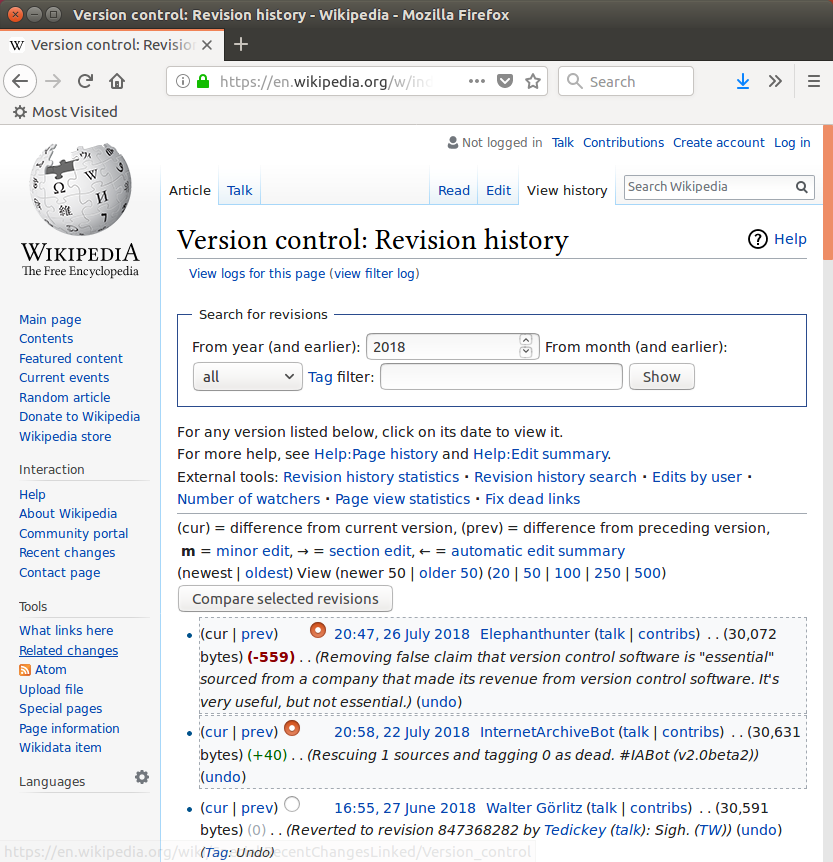
\includegraphics[width=0.9\textwidth]{images/revision-history-wikipedia.png}
   \end{figure}
\end{frame}

\begin{frame}
   \frametitle{How does version control work? Record and Playback.}
   Version control systems start with a base version of a document and
   then simply record the changes you make each step of the way.
   \begin{figure}[htbp]
      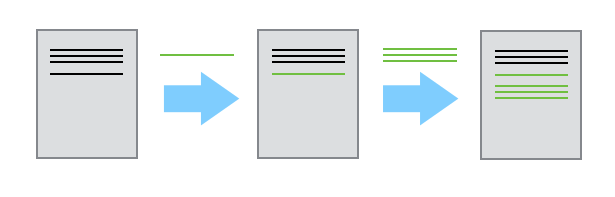
\includegraphics[width=1.0\textwidth]{images/play-changes.png}
   \end{figure}
   This allows you to rewind to start of the base document and playback
   each change you made, allowing you to recreate any version of the 
   document in its recorded history. 
\end{frame}

\begin{frame}
   \frametitle{How does version control work? Branching.}
   \begin{columns}
      \begin{column}{0.5\textwidth}
         By recording the entire history of changes to a document and 
         using the playback of those changes to recreate any version of 
         it, the management and creation of new, independent versions
         or \textit{branches} of the document itself becomes quite easy.
         \\ \ \\
         This \textit{branching} helps facilitate the collaboration 
         amongst multiple contributors to a single, shared document 
         since each contributor simply needs to record their 
         independent history of changes.
      \end{column}
      \hfill
      \begin{column}{0.5\textwidth}
         \begin{figure}[htbp]
            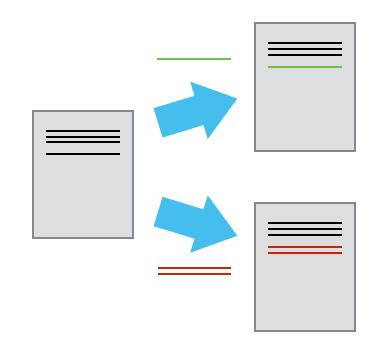
\includegraphics[width=1.0\textwidth]{images/creating-different-versions.png}
         \end{figure}
      \end{column}
   \end{columns}
\end{frame}

\begin{frame}
   \frametitle{How does version control work? Merging.}
   \begin{columns}
      \begin{column}{0.5\textwidth}
         When a contributor to a document wants to share their changes 
         with their collaborators, they simply need to \textit{merge} 
         their changes into some common branch of the document shared 
         by the team.
         \\ \ \\
         As long as there are no conflicts when the contributor's 
         independent history of changes are played back on the common, 
         shared branch of the document, the changes are
         \textit{merged} and become a part of the shared history of the
         document.
      \end{column}
      \hfill
      \begin{column}{0.5\textwidth}
         \begin{figure}[htbp]
            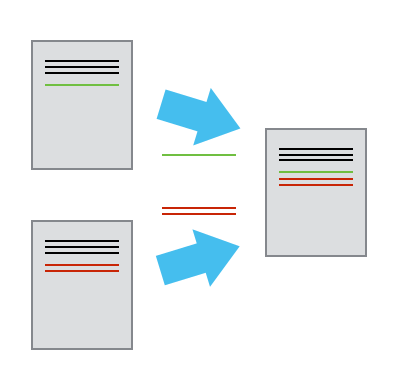
\includegraphics[width=1.0\textwidth]{images/merging-changes.png}
         \end{figure}
      \end{column}
   \end{columns}
\end{frame}

\begin{frame}
   \frametitle{Benefits of Using a Version Control System} 
   \begin{itemize}
      \setlength\itemsep{1.0em}
      \item \textbf{Archiving}: You \textit{must} regularly save the 
         changes you make.
      \item \textbf{Reproducibility}: Creating a history of saved 
         changes allows you to revert selected files or your entire 
         project back to any previous state in its recorded history.
      \item \textbf{Collaboration}: You and a team of contributors can 
         work on a project independently, but share your changes amongst 
         one another as the project takes shape.
      \item \textbf{Accountability}: Compare changes, see who last 
         modified something, and who introduced a problem and when.
      \item \textbf{Recoverability}: Each contributor has their own 
         local, recent copy of the project and its complete history,
         making it highly unlikely you'll ever lose a significant 
         portion of the project.
   \end{itemize} 
\end{frame}

\begin{frame}
   \frametitle{}
   \vspace{-1.0em}
   \begin{figure}[htbp]
      
\includegraphics[width=0.4\textwidth]{images/question-mark-sign.jpg}
   \end{figure}
\end{frame}

\begin{frame}
   \frametitle{About \texttt{git}}
   \begin{figure}[htbp]
      
\includegraphics[width=0.7\textwidth]{images/git-logo.png}
   \end{figure}
   \ \\ \ \\ 
   \begin{center}
      \url{https://git-scm.com/}
   \end{center}
\end{frame}

\begin{frame}
   \frametitle{What is \texttt{git}?}
   \begin{itemize}
      \setlength\itemsep{1.0em}
      \item \texttt{git} is a \textit{distributed} version control 
         system.
      \item \texttt{git} was designed to be \textit{simple}, 
         \textit{fast}, and \textit{fully-distributed}, with support for 
         large projects and nonlinear development workflows.
      \item \texttt{git} was originally created in 2005 by Linus 
         Torvalds and other Linux kernel developers when the free use of 
         the proprietary version control system they had been using for 
         kernel development was revoked by its copyright holder.
   \end{itemize}
\end{frame}

\begin{frame}
   \frametitle{How is \texttt{git} different? Centralized vs. Distributed}
   In general, there are two models for version control systems: \\
   \begin{itemize}
      \setlength\itemsep{1.0em}
      \item \textbf{Centralized}: Whenever you make a change and want to 
         \texttt{commit} that change, you must send it back to a 
         centralized \textit{repository} server to be tracked. However, 
         this makes sharing your changes with others who have access to 
         the server immediate once the change is committed. 
      \item \textbf{Distributed}: The process of committing changes and 
         sharing them with others broken up into a two-step process. 
         This allows you to commit changes in a 
         \textit{private repository} on your local computer, which 
         eliminates the need to be connected to a network where the 
         centralized server is accessible in order to commit a change. 
   \end{itemize}
\end{frame}

\begin{frame}
   \frametitle{How is \texttt{git} different? Private vs. Public Repositories}
   \begin{figure}[htbp]
      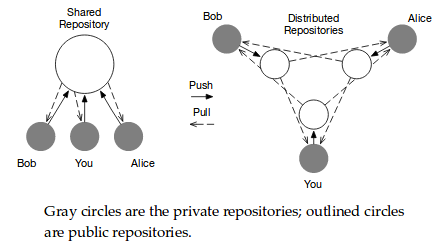
\includegraphics[width=0.7\textwidth]{images/shared-vs-distributed-repository-layout.png}
   \end{figure}
   \vspace{-1.0em}
   When using \texttt{git}, each contributer who is sharing changes with
   others on a project has at least two repositories: \\
   \begin{itemize}
      \setlength\itemsep{0.5em}
      \item a \textbf{private repository} is the one that exists on your 
         local computer and is the one you make commits to;
      \item a \textbf{public repository} is the one that you use to 
         share your changes with collaborators.
   \end{itemize}
\end{frame}

\begin{frame}
   \frametitle{The \texttt{git} workflow}
   \begin{enumerate}
      \setlength\itemsep{1.0em}
      \item Update your private repository by \texttt{fetch}ing all recent 
         changes committed by your team of collaborators from the shared 
         public repository (or their individual public repositories).
      \item Make changes and \texttt{commit} them to your private repository.
      \item Review your committed changes.
      \item Share your new changes with the team by \texttt{push}ing your 
         committed changes back to the team's shared public repository 
         (or your individual public repository)
      \item Rinse and repeat. 
   \end{enumerate}
\end{frame}

\begin{frame}
   \frametitle{}
   \vspace{-1.0em}
   \begin{figure}[htbp]
      
\includegraphics[width=0.4\textwidth]{images/question-mark-sign.jpg}
   \end{figure}
\end{frame}

\begin{frame}
   \frametitle{Getting Started with \texttt{git}}
   \begin{figure}[htbp]
      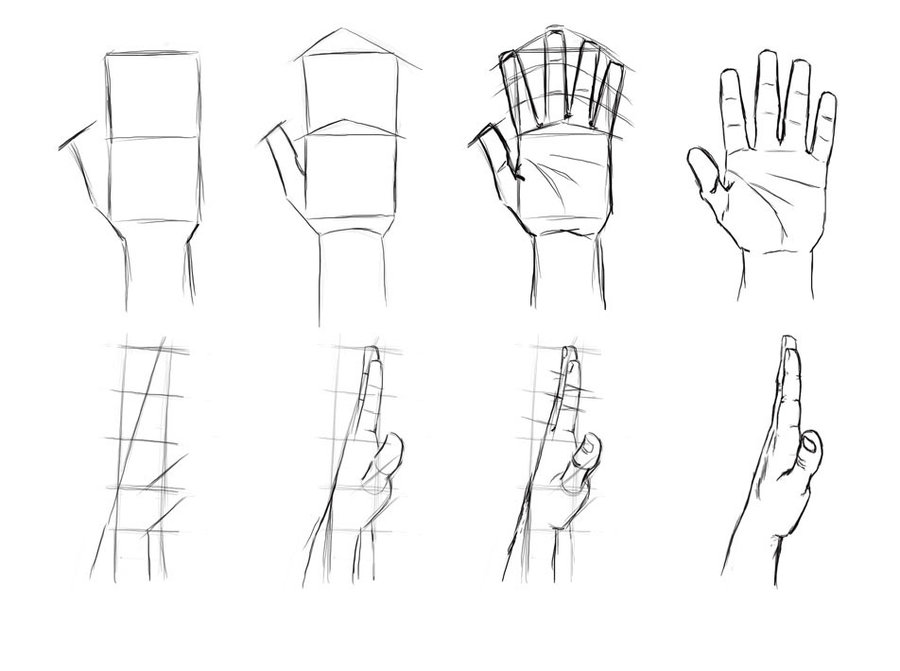
\includegraphics[width=0.7\textwidth]{images/hands-on-tutorial-by-masterss.jpg}
   \end{figure}
\end{frame}

\begin{frame}
   \frametitle{Installing \texttt{git} on Linux}
   If you want to install \texttt{git} on a Linux-based system, you 
   should be able to do so via your operating system's standard package
   management tool. 
   \\ \ \\
   For example, on any RPM-based Linux distribution, such as Fedora, 
   RHEL, or CentOS, you can use \texttt{dnf}: 
   \\ \ \\
   \hspace{1.0em}\texttt{\$ sudo dnf install git-all}
   \\ \ \\
   On any Debian-based distribution, such as Ubuntu, try \texttt{apt}: 
   \\ \ \\
   \hspace{1.0em}\texttt{\$ sudo apt install git-all} 
\end{frame}

\begin{frame}
   \frametitle{Installing \texttt{git} on Mac OS X}
   There are several ways to install \texttt{git} on your Mac. Probably 
   the easiest way is to install the Xcode Command Line Tools, which you 
   can do by simply trying to run \texttt{git} from the Terminal:
   \\ \ \\
   \hspace{1.0em}\texttt{\$ git --version}
   \\ \ \\
   If not already installed, you should be prompted to install it. 
   \\ \ \\
   If the above option does not work or you need a more up-to-date 
   version of \texttt{git}, you can always install it via a binary 
   installer maintained by the \texttt{git} team, which is available for
   download at: \\
   \begin{center}
      \url{https://git-scm.com/download/mac}
   \end{center}
\end{frame}

\begin{frame}
   \frametitle{Installing \texttt{git} on Windows}
   There are also a few ways to install \texttt{git} under Windows 
   operating systems. However, the official build is available for 
   download on the \texttt{git} website. If you go to \\
   \begin{center}
      \url{http://git-scm.com/download/win}
   \end{center}
   the download should start automatically.
   \\ \ \\
   Note: This is a project called ``\texttt{git} for Windows'', which is
   separate from \texttt{git} itself. Please see \\
   \begin{center}
      \url{https://gitforwindows.org/}
   \end{center}
    for more information.
\end{frame}

\begin{frame}
   \frametitle{Setting up \texttt{git} with \texttt{git} \texttt{config}}
   When we start using \texttt{git} for the first time on a new 
   computer, there are always a few things we need to configure
   before we begin working with \texttt{git}. 
   \\ \ \\
   The \texttt{git} \texttt{config} command lets you look up and set 
   configuration variables that control all aspects of how \texttt{git} 
   works.
\end{frame}

\begin{frame}
   \frametitle{Setting up \texttt{git} with \texttt{git} \texttt{config}}
   These configuration variables may be stored in a few different places
   on your system: \\
   \begin{enumerate}
      \setlength\itemsep{1.0em}
      \item \texttt{/etc/gitconfig}: This file contains configuration
         variables applied to every user on the system and all of their
         repositories.
      \item \texttt{{\fontfamily{ptm}\selectfont\texttildelow}/.gitconfig}: 
         This file contains configuration variables that apply only to 
         you and \textbf{all} of your repositories on the system.
      \item \texttt{{\fontfamily{ptm}\selectfont\texttildelow}/path/to/your/repo/.git/config}: This file contains configuration variables that 
         apply only to this repository.
   \end{enumerate}
\end{frame}

\begin{frame}
   \frametitle{Setting up your identity with \texttt{git} \texttt{config}}
   The first configuration variables you should set right after you install 
   \texttt{git} for the first time are your \texttt{user.name} and 
   \texttt{user.email} variables, which identify who you are and how to 
   contact you. 
   \\ \ \\
   \texttt{\hspace{1.0em}\$ git config --global user.name "Marty Kandes" \\
           \hspace{1.0em}\$ git config --global user.email "mkandes@sdsc.edu"}
   \\ \ \\
   These configuration variables are important because this information 
   is included in every \texttt{git} \texttt{commit} you make in order to 
   provide a history of who made what changes.
   \\ \ \\
   Note: The \texttt{--global} option used here places the values of 
   these configuration variables in your personal 
   \texttt{{\fontfamily{ptm}\selectfont\texttildelow}/.gitconfig}.
\end{frame}

\begin{frame}
   \frametitle{Setting up your text editor with \texttt{git} \texttt{config}}
   After you've set up your identity, you can configure the default text 
   editor that will be used by \texttt{git} when you need to edit a 
   \texttt{commit} message, etc.
   \\ \ \\
   For example, if you want to use a different text editor, such as 
   Emacs, you can type the following:
   \\ \ \\
   \texttt{\hspace{1.0em}\$ git config --global core.editor "emacs"}
   \\ \ \\
   If not configured, \texttt{git} will use your system's default editor.
   On Windows, you'll likely want to use Notepad++ as your editor.
\end{frame}

\begin{frame}
   \frametitle{Setting up colors with \texttt{git} \texttt{config}}
   In addition to your identity and default text editor, you'll also 
   want to make sure that you turn on color highlighting wherever 
   possible in \texttt{git}'s user interface. You can do so with the 
   following command:
   \\ \ \\
   \texttt{\hspace{1.0em}\$ git config --global color.ui "auto"}
\end{frame}

\begin{frame}
   \frametitle{Checking your \texttt{git} \texttt{config}}
   To check the configuration variables you've set in your 
   \texttt{git} \texttt{config}, you can run the command
   \\ \ \\
   \texttt{\hspace{1.0em}\$ git config --list}
   \\ \ \\
   to list all of the variable values. 
   \\ \ \\
   If you only need to check one variable in the configuration, you can
   always replace the \texttt{--list} option with the name of the 
   configuration variable itself. For example, if you wanted to check 
   the value of \texttt{user.email} you've set, you'd run the command:
   \\ \ \\
   \texttt{\hspace{1.0em}\$ git config user.email}
\end{frame}


\begin{frame}
   \frametitle{Getting \texttt{git} \texttt{help}}
   If you ever need \texttt{help} while using \texttt{git}, you can 
   access the comprehensive manual page (manpage) for any \texttt{git} 
   command via the \texttt{git} \texttt{help} command:
   \\ \ \\
   \texttt{\hspace{1.0em}\$ git help <command>}
   \\ \ \\
   If you only need a quick reference to the options available for a 
   given \texttt{git} command, you can use the \texttt{-h} or 
   \texttt{--help} options appended to the command itself:
   \\ \ \\
   \texttt{\hspace{1.0em}\$ git <command> -h} \\
   \texttt{\hspace{1.0em}\$ git <command> --help}
\end{frame}

\begin{frame}
   \frametitle{}
   \vspace{-1.0em}
   \begin{figure}[htbp]
      
\includegraphics[width=0.4\textwidth]{images/question-mark-sign.jpg}
   \end{figure}
\end{frame}

\begin{frame}
   \frametitle{Working with \texttt{git}}
   \begin{figure}[htbp]
      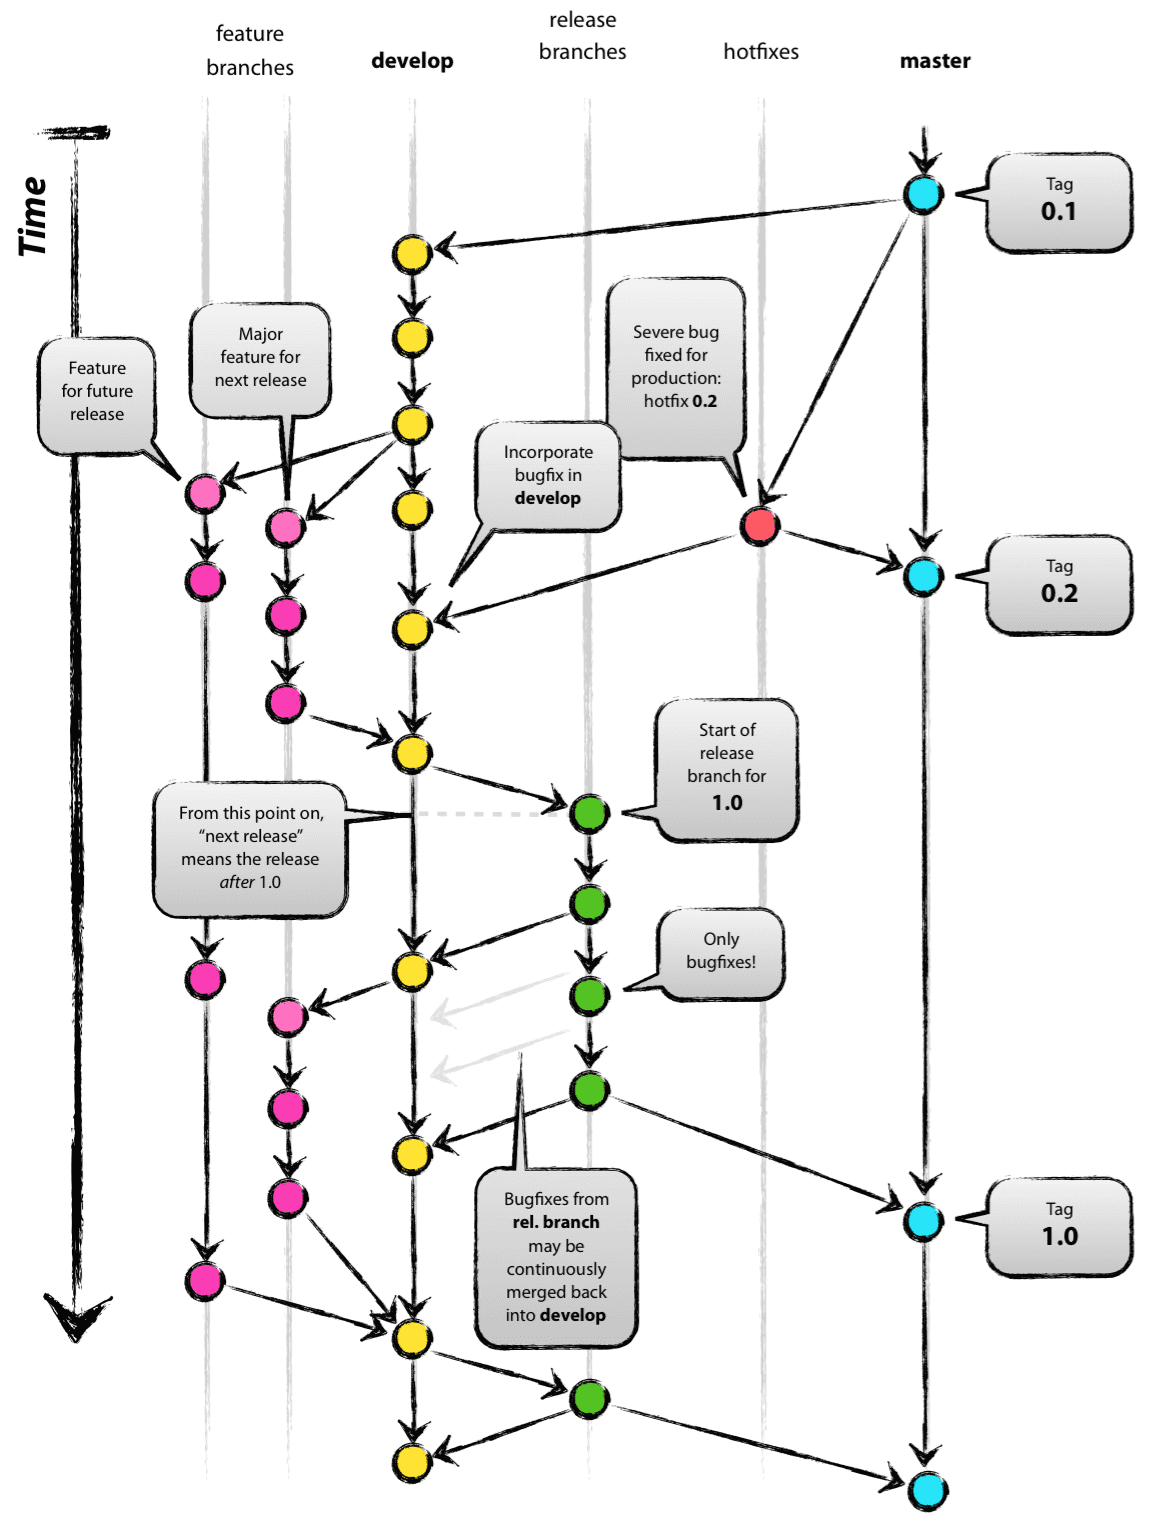
\includegraphics[width=0.5\textwidth]{images/gitflow-model.png}
   \end{figure}
\end{frame}

\begin{frame}
   \frametitle{Creating your first \texttt{git} repository with \texttt{git} \texttt{init}}
   If you have a project on your local system that is not currently
   under version control and you want to start tracking it \texttt{git},
   you can create a git repository for that project by first going to
   that project's directory
   \\ \ \\
   \texttt{\hspace{1.0em}\$ cd /path/to/your/project}
   \\ \ \\
   and then typing the command:
   \\ \ \\
   \texttt{\hspace{1.0em}\$ git init}
   \\ \ \\
   This creates a new subdirectory named \texttt{.git} in the project 
   directory where the repository will live. If you ever want to stop 
   tracking the project with \texttt{git}, you simply need to delete 
   this subdirectory.
\end{frame}

\begin{frame}
   \frametitle{Creating your first \texttt{git} repository with \texttt{git} \texttt{init}}
   \begin{figure}[htbp]
      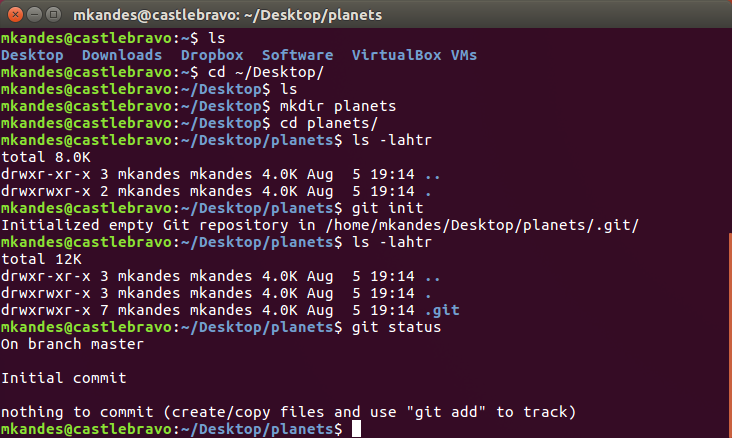
\includegraphics[width=1.0\textwidth]{images/git-init.png}
   \end{figure}
\end{frame}

\begin{frame}
   \frametitle{Checking the state your repository with \texttt{git} \texttt{status}}
   Each file in your repository's working directory may take on one of 
   a few different states. The main tool you use to determine which files
   are in which state is with the command:
   \\ \ \\
   \texttt{\hspace{1.0em}\$ git status}
\end{frame}

\begin{frame}
   \frametitle{Different states of a file in a \texttt{git} repository}
   \begin{figure}[htbp]
      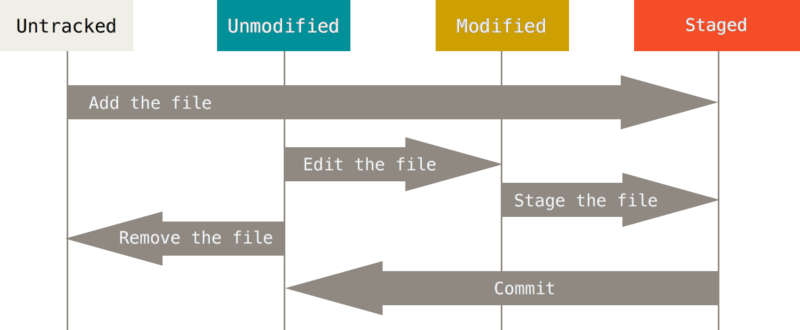
\includegraphics[width=0.8\textwidth]{images/git-file-lifecycle.png}
   \end{figure}
   There are two primary file states you will find in your repository: \\
   \begin{enumerate}
      \setlength\itemsep{0.5em}
      \item \textbf{Tracked files} are all of the files that 
         \texttt{git} already knows about and has under version control; 
         they have secondary states, where they can be either 
         \textit{unmodified}, \textit{modified}, or \textit{staged}. 
      \item \textbf{Untracked files} are everything else --- any files 
         in your project's working directory not yet under version 
         control.
   \end{enumerate}
\end{frame}

\begin{frame}
   \frametitle{Adding files to your \texttt{git} repository with \texttt{git} \texttt{add}}
   \begin{figure}[htbp]
      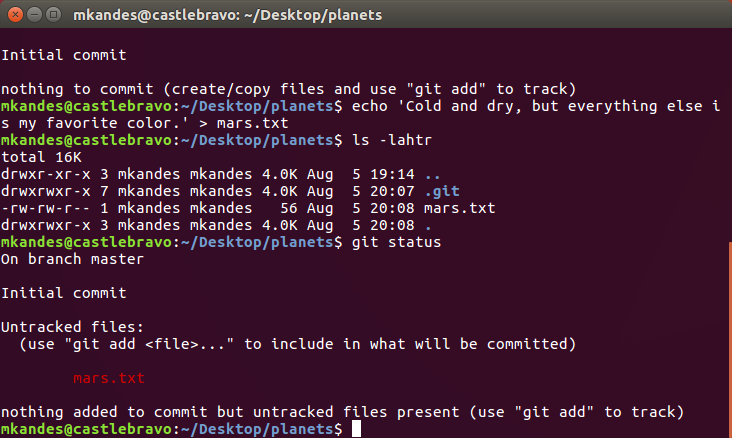
\includegraphics[width=1.0\textwidth]{images/git-untracked-file.png}
   \end{figure}
\end{frame}

\begin{frame}
   \frametitle{Adding files to your \texttt{git} repository with \texttt{git} \texttt{add}}
   \begin{figure}[htbp]
      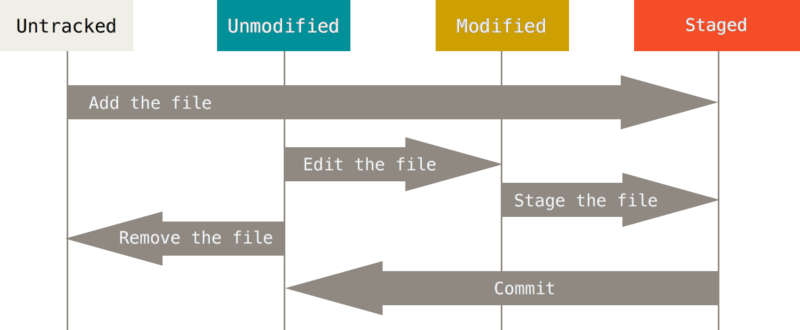
\includegraphics[width=0.8\textwidth]{images/git-file-lifecycle.png}
   \end{figure}
   To begin tracking a new file in your project's working directory, you 
   must first \textit{stage} the new file to be committed to the 
   repository with the command:
   \\ \ \\
   \texttt{\hspace{1.0em}\$ git add <path/to/file/filename>}
   \\ \ \\
   If you run \texttt{git} \texttt{status} again, you should see that 
   the newly added file is now tracked and staged to be committed.
\end{frame}

\begin{frame}
   \frametitle{Adding files to your \texttt{git} repository with \texttt{git} \texttt{add}}
   \begin{figure}[htbp]
      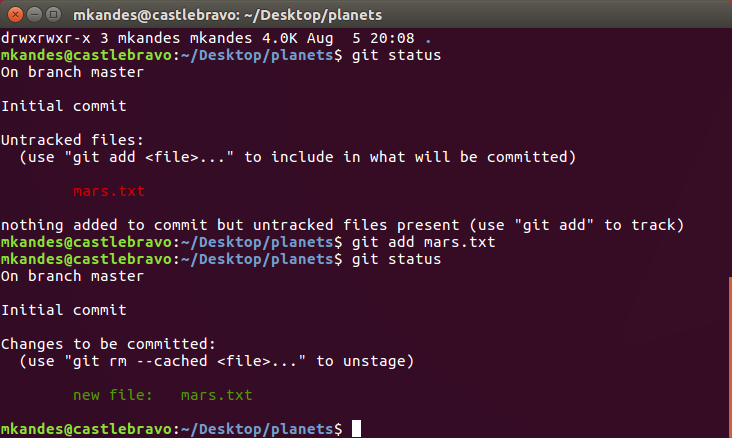
\includegraphics[width=1.0\textwidth]{images/git-add.png}
   \end{figure}
\end{frame}

\begin{frame}
   \frametitle{Committing changes with \texttt{git} \texttt{commit}}
   \begin{figure}[htbp]
      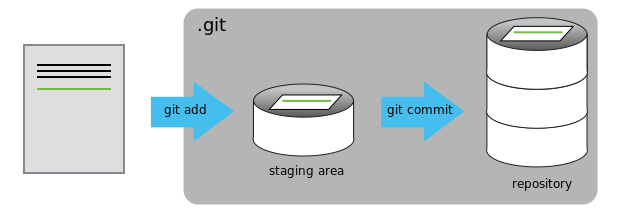
\includegraphics[width=0.8\textwidth]{images/git-staging-area.png}
   \end{figure}
   Changes to files in your repository are tracked through commits, 
   which you make with the 
   \\ \ \\
   \texttt{\hspace{1.0em}\$ git commit}
   \\ \ \\ 
   command. Prior to most commits, you need to stage the files whose 
   changes you want to commit using the \texttt{git} \texttt{add} 
   command.
\end{frame}

\begin{frame}
   \frametitle{Writing a commit message}
   Each commit requires a commit message. They provide the 
   \textit{context} about \textit{why} a change was made. This may be 
   to inform other collaborators working on the project about the change 
   or, more often, to remind yourself why you made the change.
   \\ \ \\
   How you choose to format your commit messages is up to you and your 
   team. But if you need some guidance, here are seven rules to writing a 
   great \texttt{git} commit message: \\
   \begin{center}
      \url{https://chris.beams.io/posts/git-commit/}
   \end{center}
\end{frame}

\begin{frame}
   \frametitle{Writing a commit message}
   \begin{figure}[htbp]
      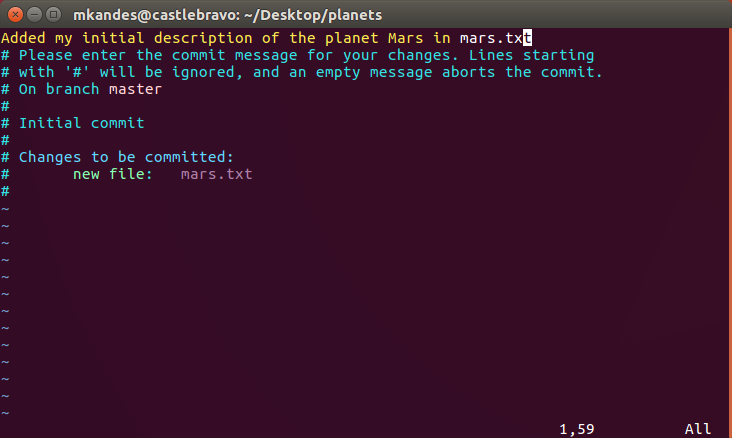
\includegraphics[width=1.0\textwidth]{images/git-commit-message.png}
   \end{figure}
\end{frame}

\begin{frame}
   \frametitle{Committing changes with \texttt{git} \texttt{commit}}
   \begin{figure}[htbp]
      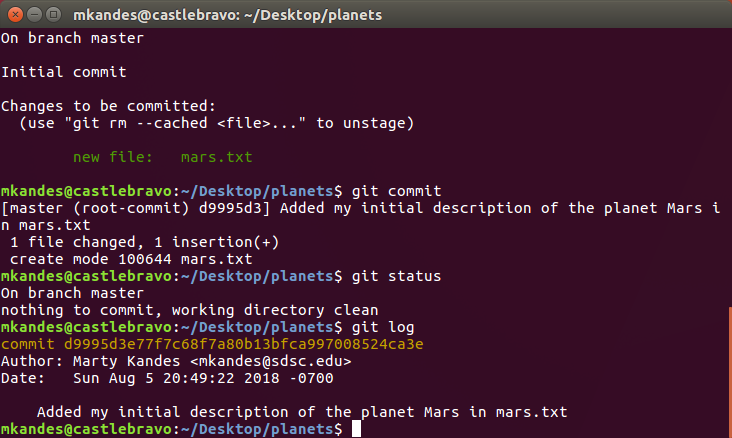
\includegraphics[width=1.0\textwidth]{images/git-after-commit.png}
   \end{figure}
\end{frame}

\begin{frame}
   \frametitle{Viewing your commit history with \texttt{git} \texttt{log}}
   The power of \texttt{git} is that it tracks the changes to files in 
   your project over time. You can use the
   \\ \ \\
   \texttt{\hspace{1.0em}\$ git log}
   \\ \ \\
   command to view that history.
   \\ \ \\
   In the standard output of the \texttt{git} \texttt{log} command, you
   will see the commit ID of each commit, the author who made it, the 
   date it was committed, and the commit message explaining the reason 
   for the change(s).
   \\ \ \\
   By default, the \texttt{git} \texttt{log} command will list commit 
   history in reverse chronological order. 
\end{frame}

\begin{frame}
   \frametitle{Let's add some more files and make some changes ...}
   \begin{figure}[htbp]
      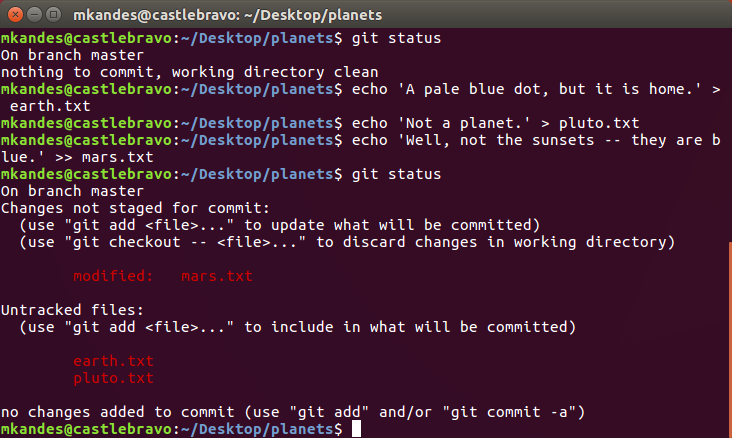
\includegraphics[width=1.0\textwidth]{images/git-adding-more-files-and-some-changes.png}
   \end{figure}
\end{frame}

\begin{frame}
   \frametitle{... then begin tracking the new files and stage the changes for the next commit ...}
   \begin{figure}[htbp]
      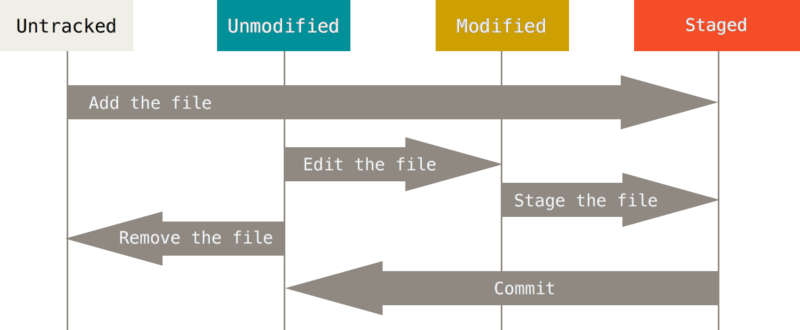
\includegraphics[width=1.0\textwidth]{images/git-file-lifecycle.png}
   \end{figure}
\end{frame}

\begin{frame}
   \frametitle{Staging new, untracked files and committing them ...}
   \begin{figure}[htbp]
      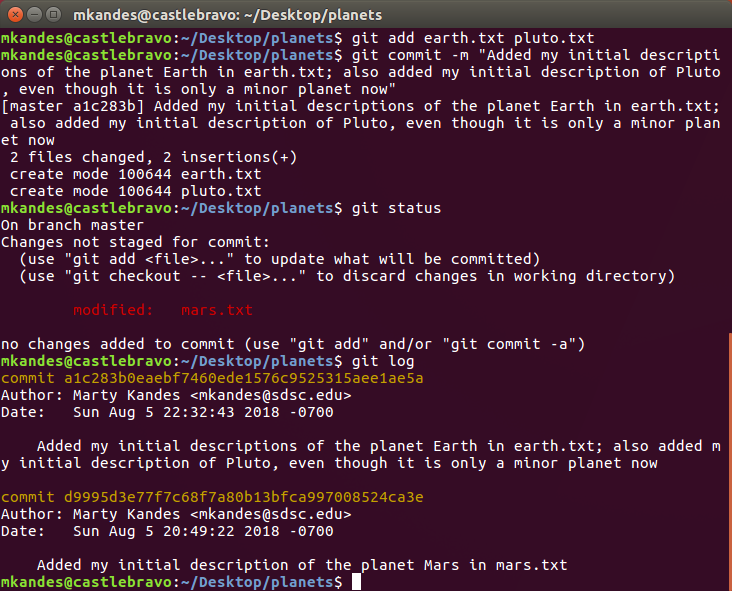
\includegraphics[width=1.0\textwidth]{images/git-add-and-commit-more-new-files.png}
   \end{figure}
\end{frame}

\begin{frame}
   \frametitle{Comparing differences with \texttt{git} \texttt{diff}}
   While \texttt{git} \texttt{log} provides you with information about a 
   commit -- who made it, when they made it, and why they made it --- 
   sometimes looking at the specific changes made to the files themselves 
   is what's more important.
   \\ \ \\
   You can use the 
   \\ \ \\
   \texttt{\hspace{1.0em}\$ git diff}
   \\ \ \\
   command to see the changes to any \textit{modified} files in your working 
   directory before you stage them to be committed.
\end{frame}

\begin{frame}
   \frametitle{Comparing differences with \texttt{git} \texttt{diff}}
   \begin{figure}[htbp]
      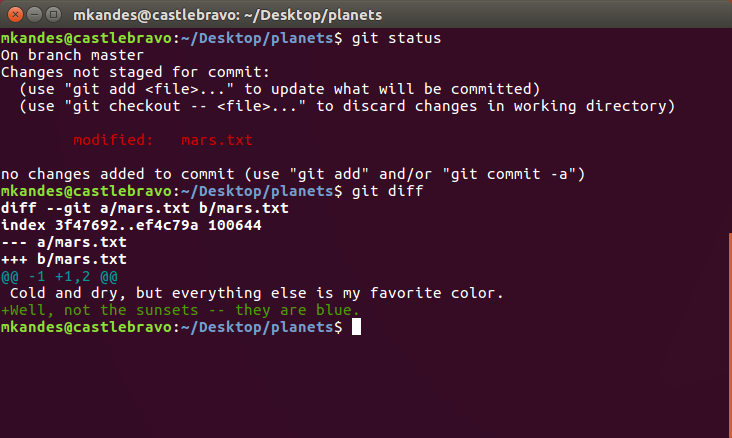
\includegraphics[width=1.0\textwidth]{images/git-diff.png}
   \end{figure}
\end{frame}

\begin{frame}
   \frametitle{Breaking down a \texttt{git} \texttt{diff} line-by-line}
   \begin{enumerate}
      \setlength\itemsep{1.0em}
      \item The first line tells us that \texttt{git} is comparing the 
         old and new versions of the file with the \texttt{diff} command.
      \item The second line tells us exactly which versions of the file 
         are being compared.
      \item The next two lines once again show the name of the file 
         being changed.
      \item The remaining lines show us the actual differences between 
         the files and the lines on which they occur, with the \texttt{+} 
         character in the first column showing where we added a new line 
         of text.
   \end{enumerate}
\end{frame}

\begin{frame}
   \frametitle{After reviewing our change, it's time to commit it ...}
   \begin{figure}[htbp]
      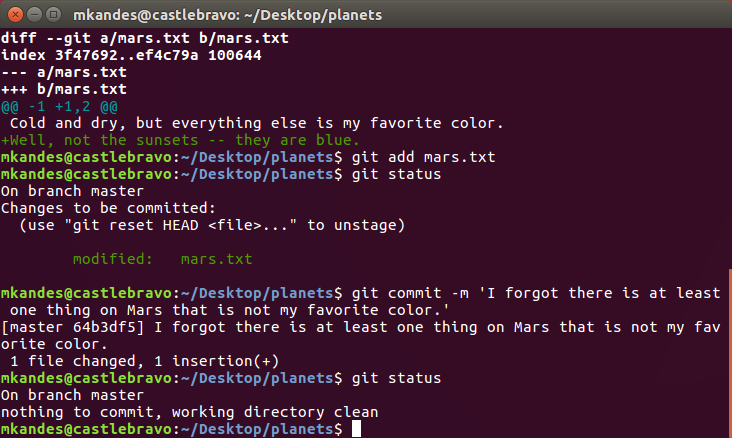
\includegraphics[width=1.0\textwidth]{images/git-add-and-commit-modified-file.png}
   \end{figure}
\end{frame}

\begin{frame}
   \frametitle{Moving files and directories with \texttt{git} \texttt{mv}}
   Performing tasks such as reorganizing files under new directories, 
   changing filenames, and so on requires that files or sometimes entire 
   directories get moved from once place to another in your repository. 
   \\ \ \\
   You can move a file (or directory) into another one with the command:
   \\ \ \\
   \texttt{\hspace{1.0em}\$ git mv <path/to/old/fname> <path/to/newfname>}
   \\ \ \\
   \texttt{git} will stage the change for you after you call 
   \texttt{git} \texttt{mv}. You must then call \texttt{git} 
   \texttt{commit} afterwards to make the move permanent.
\end{frame}

\begin{frame}
   \frametitle{Moving files and directories with \texttt{git} \texttt{mv}}
   \begin{figure}[htbp]
      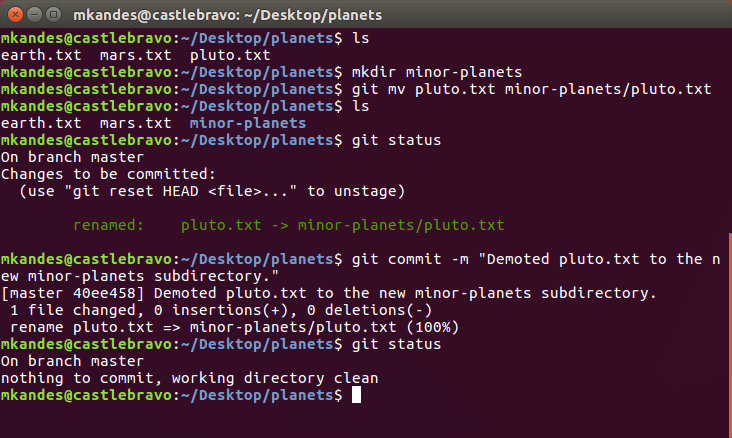
\includegraphics[width=1.0\textwidth]{images/git-mv.png}
   \end{figure}
\end{frame}

\begin{frame}
   \frametitle{Removing files and directories with \texttt{git} \texttt{rm}}
   Files and directories in your repository sometimes outlive their 
   usefulness. When this occurs, you can tell \texttt{git} to stop 
   tracking changes to these files and remove them from the working tree 
   of your repository --- your copy of the repository at a particular 
   point in its commit history; normally at the last commit.
   \\ \ \\
   To an remove an outdated file (or a directory) from the working tree 
   of your repository, you use the command:
   \\ \ \\
   \texttt{\hspace{1.0em}\$ git rm -- <path/to/file/filename>}
   \\ \ \\
   This \textbf{does not} remove the file from your repository's 
   history; it only removes it from your working tree going forward
   \\ \ \\
   Like other \texttt{git} actions, you must run \texttt{git} 
   \texttt{commit} after \texttt{git} \texttt{rm} to finalize the 
   change.
\end{frame}

\begin{frame}
   \frametitle{Removing files and directories with \texttt{git} \texttt{rm}}
   \begin{figure}[htbp]
      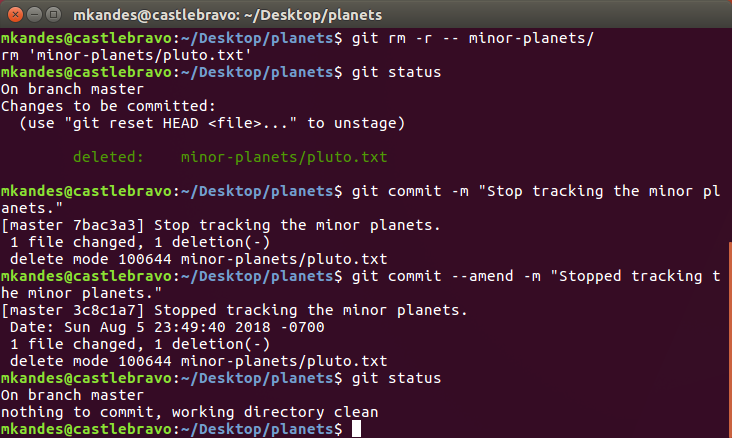
\includegraphics[width=1.0\textwidth]{images/git-rm.png}
   \end{figure}
\end{frame}

\begin{frame}
   \frametitle{Creating and switching between \texttt{git} \texttt{branch}es}
   When you want to begin modifying the contents of your repository, 
   but only want to do so to a limited subset of the files in it, you 
   can begin using the \textit{branching} and \textit{merging} 
   mechanisms of \texttt{git}.
   \\ \ \\
   To create a new \textit{branch} in your repository, you use the command:
   \\ \ \\
   \texttt{\hspace{1.0em}\$ git branch <branch-name>}
   \\ \ \\
   To then begin working on this new branch, you must switch over to this branch of this project using the command:
   \\ \ \\
   \texttt{\hspace{1.0em}\$ git checkout <branch-name>}
   \\ \ \\
   The default branch in every \texttt{git} repository is the 
   \texttt{master} branch.
\end{frame}
 

\begin{frame}
   \frametitle{Creating and switching between \texttt{git} \texttt{branch}es}
   \begin{figure}[htbp]
      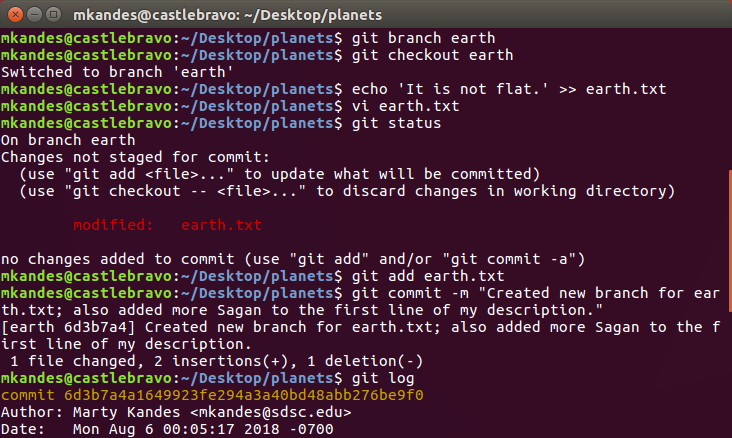
\includegraphics[width=1.0\textwidth]{images/git-branch-and-checkout.png}
   \end{figure}
\end{frame}

\begin{frame}
   \frametitle{Creating and switching between \texttt{git} \texttt{branch}es}
   \begin{figure}[htbp]
      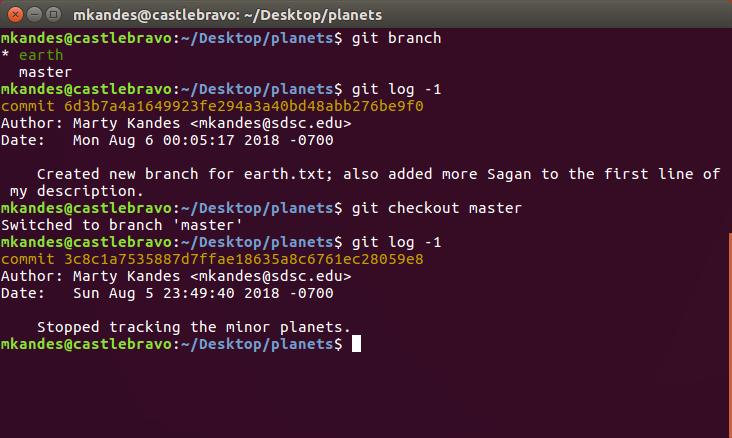
\includegraphics[width=1.0\textwidth]{images/git-branch-compare-with-master.png}
   \end{figure}
\end{frame}

\begin{frame}
   \frametitle{Creating and switching between \texttt{git} \texttt{branch}es}
   \begin{figure}[htbp]
      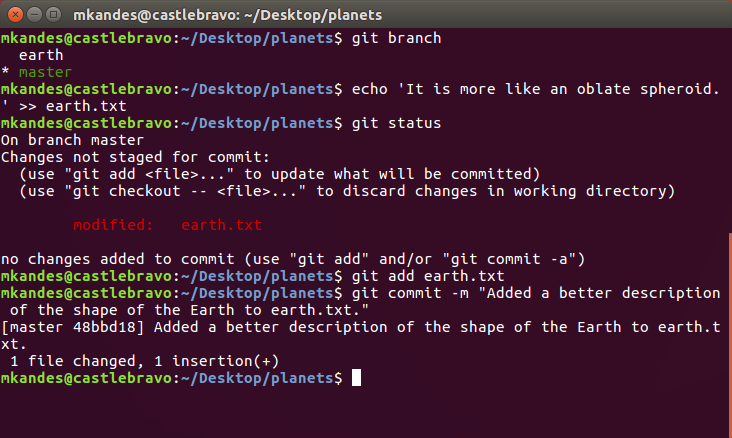
\includegraphics[width=1.0\textwidth]{images/git-branch-modifying-earth-on-master.png}
   \end{figure}
\end{frame}

\begin{frame}
   \frametitle{Merging commits between branches with \texttt{git} \texttt{merge}}
   Once you and/or your collaborators have made changes on a project in 
   different branches, at some point you'll want to \textit{merge} your 
   changes together. 
   \\ \ \\
   To \textit{merge} the changes from different branches, you first need
   to \textit{checkout} the branch you want the changes to be merged into.
   \\ \ \\
   \texttt{\hspace{1.0em}\$ git checkout <branch-name>}
   \\ \ \\
   You then select the changes from another branch to be merged into this 
   current branch. 
   \\ \ \\
   \texttt{\hspace{1.0em}\$ git merge <branch-name-to-be-merged>}
   \\ \ \\
   Note, however, if there is a \textit{conflict} between the content 
   the two branches, you must first resolve these conflicts prior to 
   committing the merge.
\end{frame}

\begin{frame}
   \frametitle{Merging commits between branches with \texttt{git} \texttt{merge}}
   \begin{figure}[htbp]
      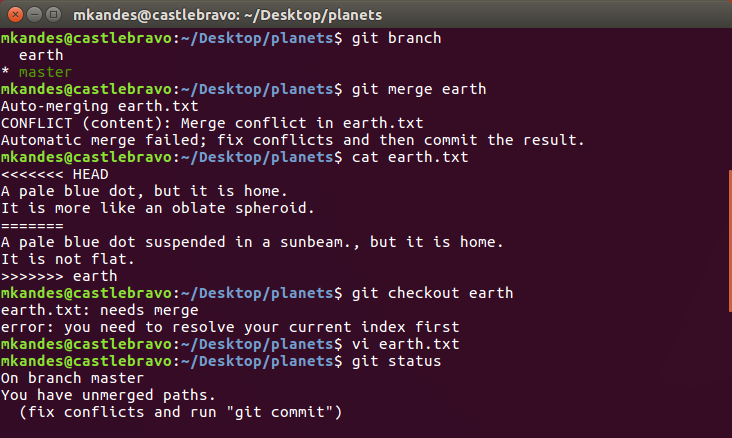
\includegraphics[width=1.0\textwidth]{images/git-merge-with-conflict-part1.png}
   \end{figure}
\end{frame}

\begin{frame}
   \frametitle{Merging commits between branches with \texttt{git} \texttt{merge}}
   \begin{figure}[htbp]
      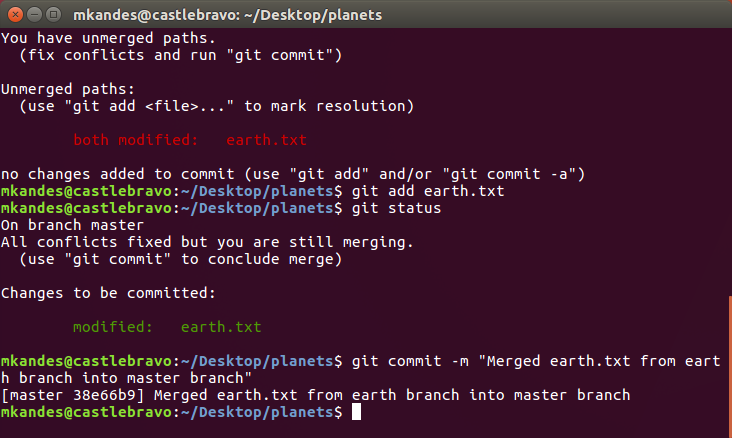
\includegraphics[width=1.0\textwidth]{images/git-merge-with-conflict-part2.png}
   \end{figure}
\end{frame}

\begin{frame}
   \frametitle{Merging commits between branches with \texttt{git} \texttt{merge}}
   \begin{figure}[htbp]
      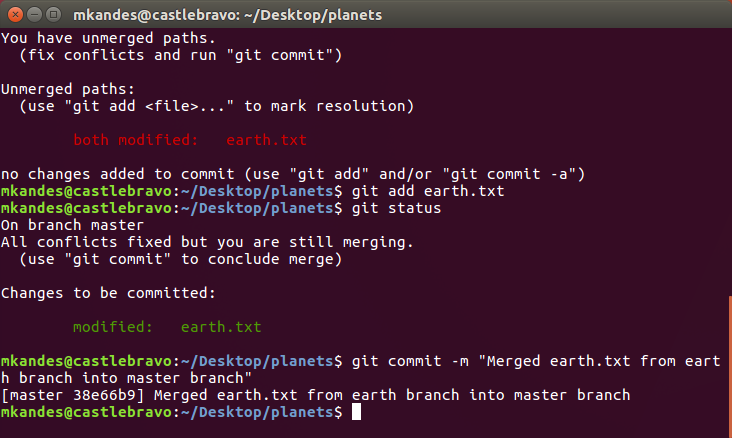
\includegraphics[width=1.0\textwidth]{images/git-merge-with-conflict-part2.png}
   \end{figure}
\end{frame}

\begin{frame}
   \frametitle{}
   \vspace{-1.0em}
   \begin{figure}[htbp]
      
\includegraphics[width=0.4\textwidth]{images/question-mark-sign.jpg}
   \end{figure}
\end{frame}

\begin{frame}
   \frametitle{Getting Started with GitHub}
   \begin{figure}[htbp]
      
\includegraphics[width=0.7\textwidth]{images/github-logo.jpg}
   \end{figure}
   \ \\ \ \\
   \begin{center}
      \url{https://github.com/}
   \end{center}
\end{frame}

\begin{frame}
   \frametitle{Your GitHub Profile}
   \begin{figure}[htbp]
      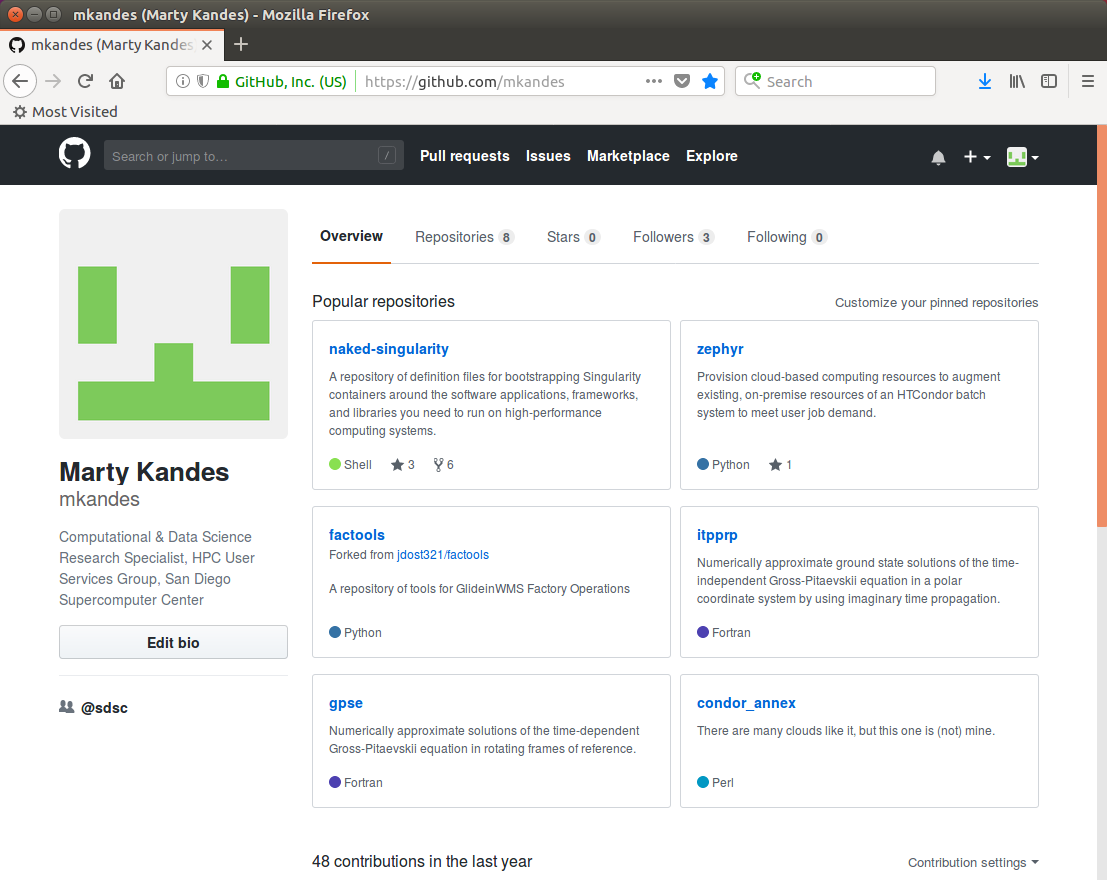
\includegraphics[width=1.0\textwidth]{images/my-github-repo.png}
   \end{figure}
\end{frame}

\begin{frame}
   \frametitle{Creating a New GitHub Repository}
   \begin{figure}[htbp]
      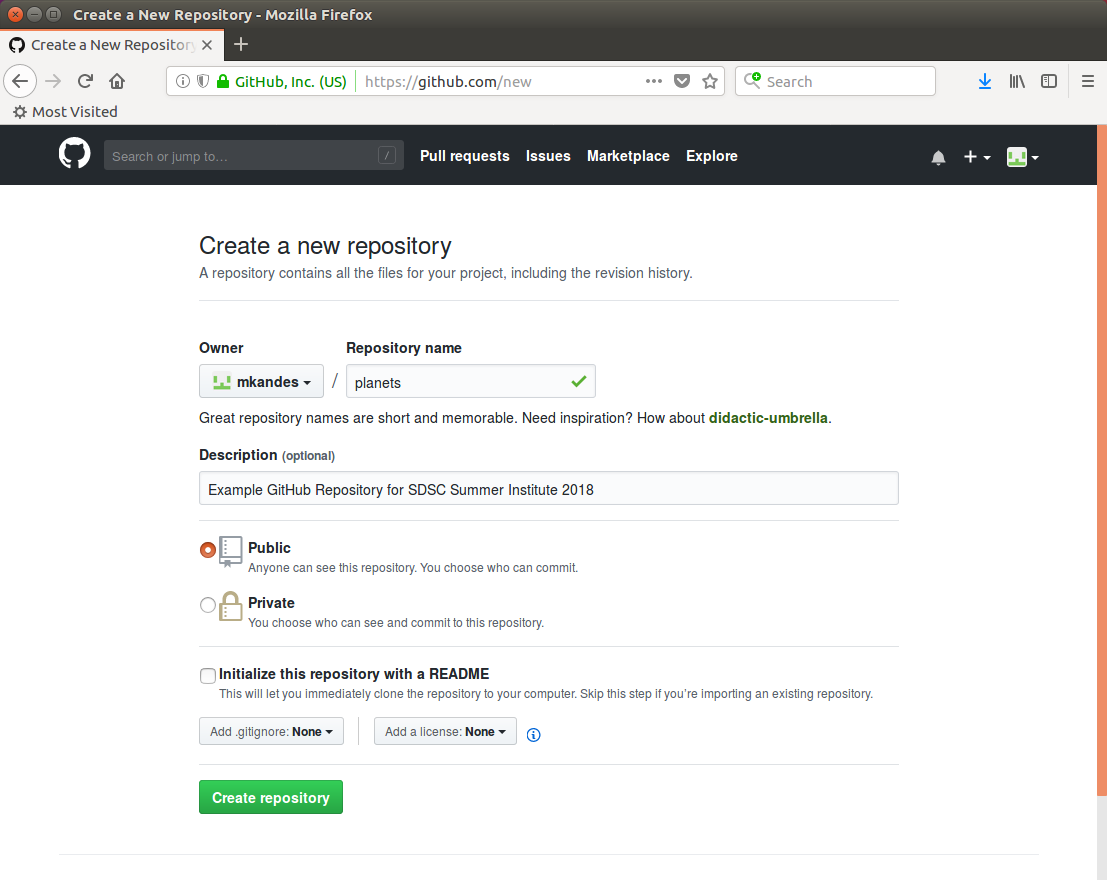
\includegraphics[width=1.0\textwidth]{images/github-create-new-repo.png}
   \end{figure}
\end{frame}

\begin{frame}
   \frametitle{Creating a New GitHub Repository}
   \begin{figure}[htbp]
      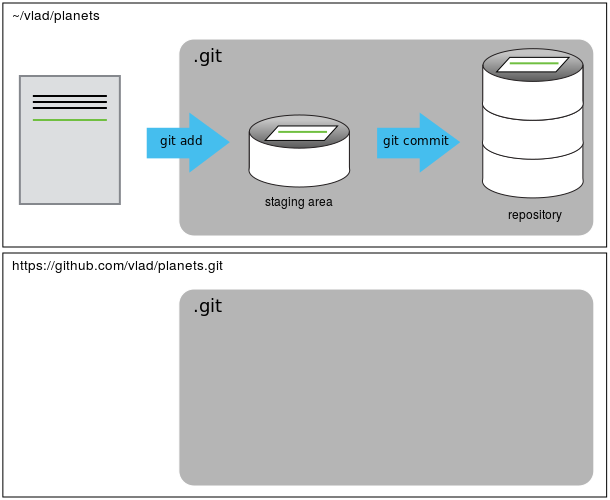
\includegraphics[width=0.7\textwidth]{images/git-freshly-made-github-repo.png}
   \end{figure}
\end{frame}

\begin{frame}
   \frametitle{How to make your GitHub repository a \texttt{remote}}
   \begin{figure}[htbp]
      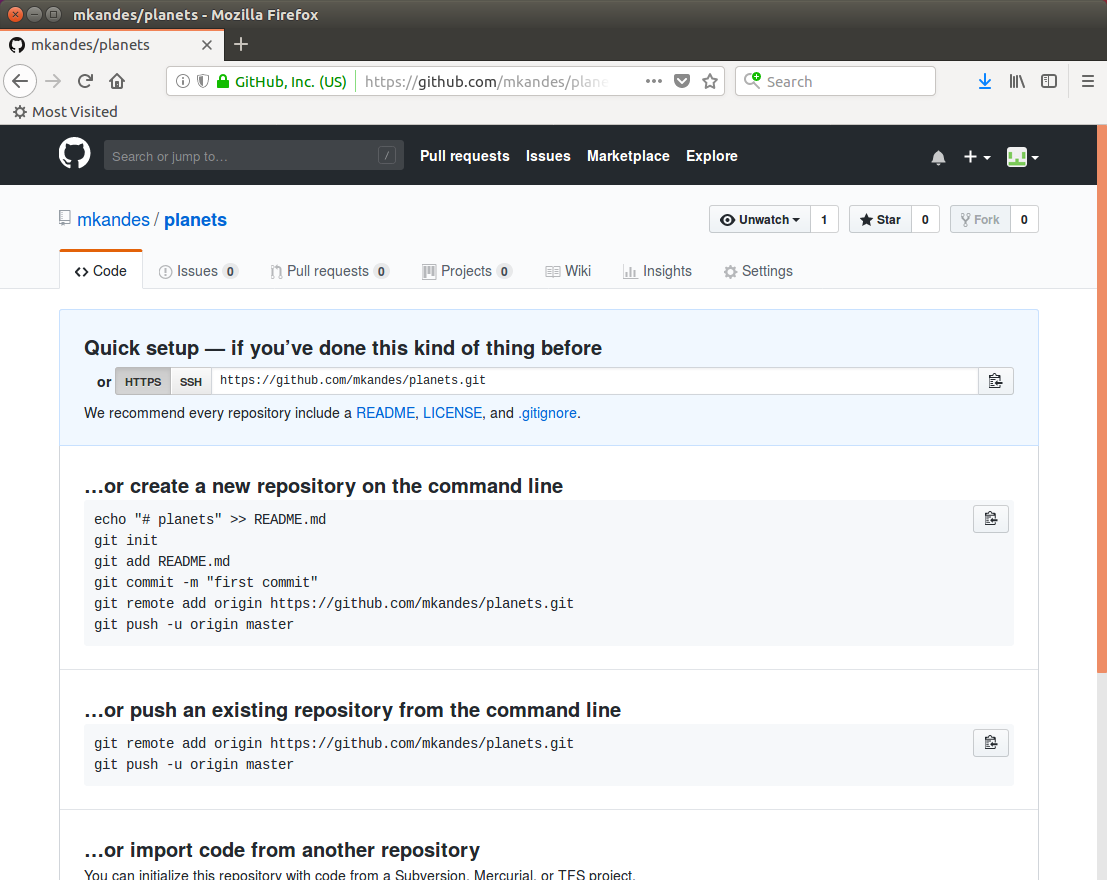
\includegraphics[width=1.0\textwidth]{images/github-how-to-setup-new-repo.png}
   \end{figure}
\end{frame}

\begin{frame}
   \frametitle{How to make your GitHub repository a \texttt{remote}}
   \begin{figure}[htbp]
      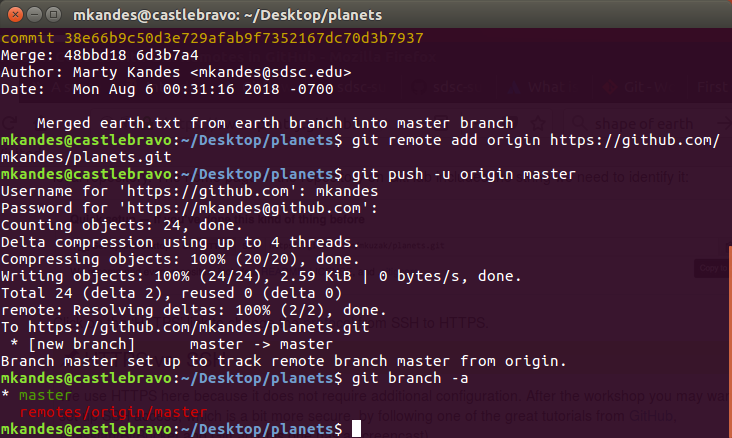
\includegraphics[width=1.0\textwidth]{images/git-add-github-remote-and-push.png}
   \end{figure}
\end{frame}

\begin{frame}
   \frametitle{Your GitHub repository after the first \texttt{git} \texttt{push}}
   \begin{figure}[htbp]
      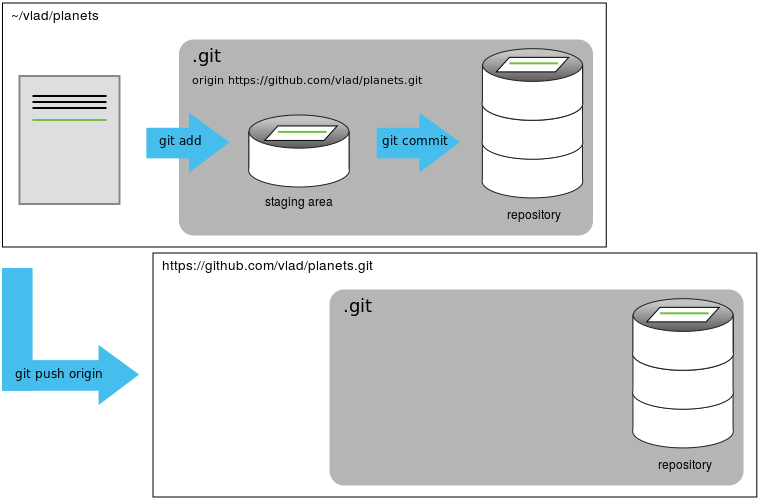
\includegraphics[width=1.0\textwidth]{images/github-repo-after-first-push-diagram.png}
   \end{figure}
\end{frame}

\begin{frame}
   \frametitle{Your GitHub repository after the first \texttt{git} \texttt{push}}
   \begin{figure}[htbp]
      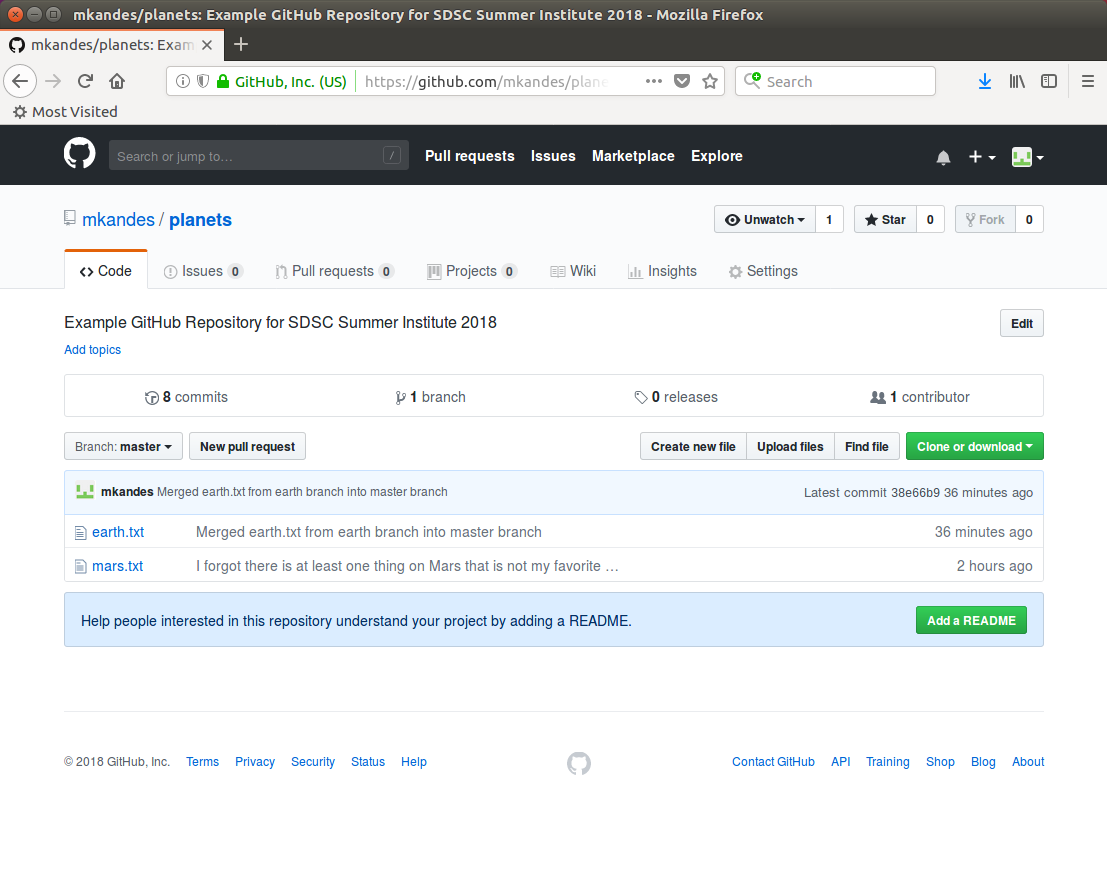
\includegraphics[width=1.0\textwidth]{images/github-repo-after-first-push-web.png}
   \end{figure}
\end{frame}

\begin{frame}
   \frametitle{Cloning a GitHub repository with \texttt{git} \texttt{clone}}
   \begin{figure}[htbp]
      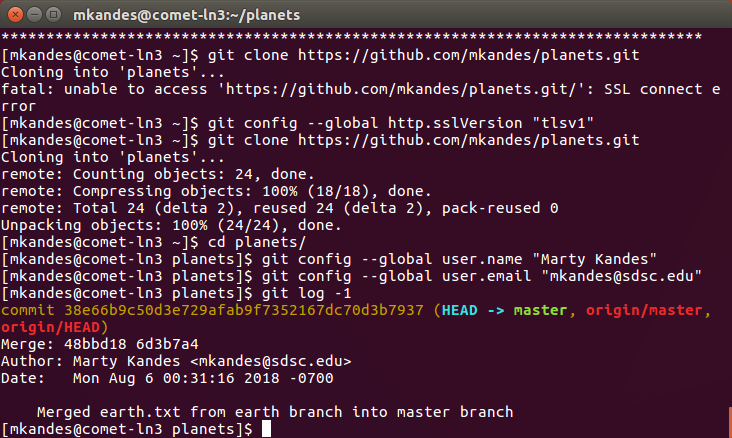
\includegraphics[width=1.0\textwidth]{images/git-clone-github-repo-to-comet.png}
   \end{figure}
\end{frame}

\begin{frame}
   \frametitle{Modify cloned repository and push changes back to GitHub}
   \begin{figure}[htbp]
      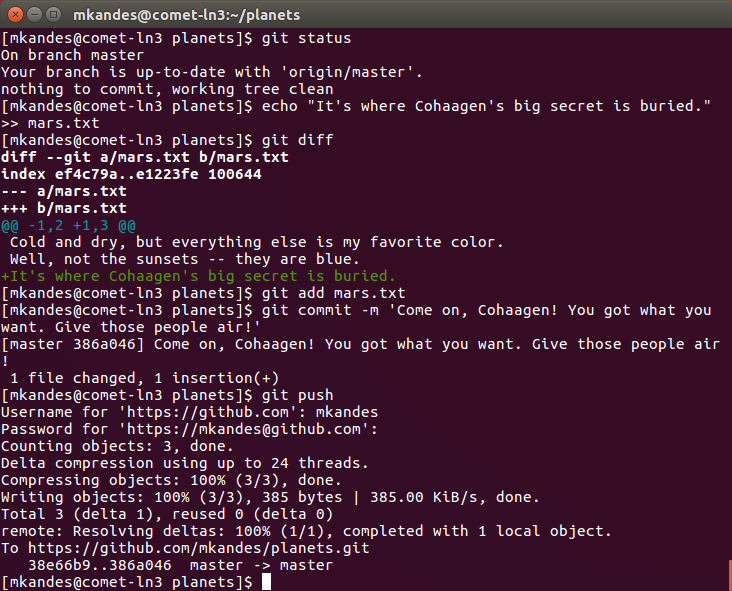
\includegraphics[width=0.9\textwidth]{images/git-push-from-comet.png}
   \end{figure}
\end{frame}

\begin{frame}
   \frametitle{GitHub repository after recent push}
   \begin{figure}[htbp]
      \includegraphics[width=1.0\textwidth]{images/github-after-push-from-comet.png}
   \end{figure}
\end{frame}

\begin{frame}
   \frametitle{Summary and Conclusion: Benefits of Version Control}
   \begin{itemize}
      \setlength\itemsep{1.0em}\footnotesize
      \item \textbf{Archiving}: You \textit{must} regularly save the
         changes you make.
      \item \textbf{Reproducibility}: Creating a history of saved
         changes allows you to revert selected files or your entire
         project back to any previous state in its recorded history.
      \item \textbf{Collaboration}: You and a team of contributors can
         work on a project independently, but share your changes amongst
         one another as the project takes shape.
      \item \textbf{Accountability}: Compare changes, see who last
         modified something, and who introduced a problem and when.
      \item \textbf{Recoverability}: Each contributor has their own
         local, recent copy of the project and its complete history,
         making it highly unlikely you'll ever lose a significant
         portion of the project.
   \end{itemize}
   \ \\
   "\textit{Version control software is very useful, but it is not essential}." \\
   \ \ \ \ \ \ \ \ \ \ \ \ \ \ \ \ \ \ \ \ \ \ \ \ \ \ \ \ \ \  \ \ \ \ \ \ \ \ \ \ \ \ \ \ \ \ \ \ \ \ \ \ \ \ -- \texttt{Elephanthunter}
\end{frame}

\begin{frame}
   \frametitle{The End}
   \begin{figure}[htbp]
      \includegraphics[width=1.0\textwidth]{images/total-recall.jpg}
   \end{figure}
\end{frame}

\begin{frame}
   \frametitle{}
   \vspace{-1.0em}
   \begin{figure}[htbp]
      \includegraphics[width=0.4\textwidth]{images/question-mark-sign.jpg}
   \end{figure}
\end{frame}

\begin{frame}
   \frametitle{References}
    \begin{itemize}
      \setlength\itemsep{1.0em}
      \item \textbf{Version Control with Git} by D.Huang and I. Gonzalez \\ 
         \url{https://swcarpentry.github.io/git-novice/}
      \item \textbf{Pragmatic Version Control Using Git} by T. Swicegood
      \item \textbf{Pro Git} by S. Chacon and B. Straub \\
         \url{https://git-scm.com/book/en/v2}
   \end{itemize}
\end{frame}

\end{document}
